\documentclass[a4paper,11pt]{jsarticle}


% 数式
\usepackage{amsmath,amsfonts}
\usepackage{bm}
\usepackage{physics}
% 画像
\usepackage[dvipdfmx]{graphicx}
% ローマ数字
\usepackage{otf}
% 単位
\usepackage{siunitx}
% 表
\usepackage{multirow}
% 化学反応
\usepackage[version=4]{mhchem}


\begin{document}

\title{電子回路論 第1回レポート}
\author{05-211525 齋藤駿一}
\date{\today}
\maketitle

\section*{課題1}
図\ref{fig:1}のような回路を設計した.
このとき,オペアンプの入力電圧は
\begin{equation}
  V_{+} = \frac{10}{11}V_1, \qquad V_{-} = \frac{1}{11}V_{\mathrm{O}} + \frac{10}{11}V_2
\end{equation}
となるので,$V_{+}=V_{-}$を解くと,
\begin{equation}
  V_{\mathrm{O}} = 10(V_1 - V_2)
\end{equation}
が得られる.

\begin{figure}[htbp]
  \centering
  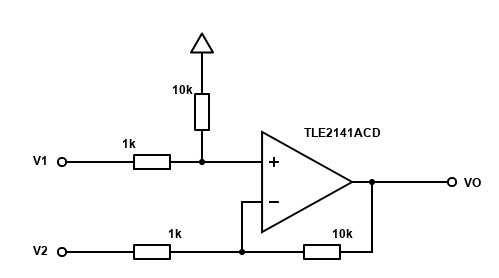
\includegraphics[width=10cm]{schemeit-project.png}
  \caption{差動増幅回路(ゲイン10倍)}
  \label{fig:1}
\end{figure}

\section*{課題2}

データシートより,オペアンプの入力オフセット電圧は室温(\SI{25}{\degreeCelsius})で$V_{\mathrm{IO}}=\SI{500}{\micro\V}$である.
これが10倍に増幅されて出力されるので,$V_1=V_2=0$のとき,
\begin{equation}
  V_{\mathrm{O}} \approx 10\times \SI{500}{\micro\V} = \SI{5}{\mV}
\end{equation}
程度のDC成分が出力される.

\section*{課題3}

データシートより,\SI{1}{\kHz}におけるノイズは\SI{10.5}{\nV/\Hz^{1/2}}である.
また,温度$T$での抵抗$R$におけるジョンソンノイズは$\sqrt{4kTR}$で与えられる.
ただし,$k$はボルツマン定数である.
本回路では,オペアンプのマイナス端子に繋がっている\SI{10}{\kohm}抵抗以外の3つの抵抗から発されるノイズがそれぞれ10倍に増幅されて出力される.
したがって,それらのノイズが独立に重なったとき,全体の振幅は2乗和をとって
\begin{equation}
  \sqrt{10\times (4kT(2\times\SI{1}{\kohm}+\SI{10}{\kohm}) + (\SI{10.5}{\nV/\Hz^{1/2}})^2) + 4kT\times\SI{10}{\kohm}} \approx \SI{57}{\nV/\Hz^{1/2}}
\end{equation}
と計算できる.

\end{document}